老早就久仰 Spark 的大名, 自己也在服务器上用 docker 搭过 Spark 集群, 做了一点简单的尝试, 但总是差点感觉, 处于盲人摸象的阶段, 对 Spark 的认识还是一团浆糊. 有幸接触到了 《大数据处理框架 Apache Spark 设计与实现》\footnote{许利杰, 方亚芬著, 电子工业出版社}, 解答了我不少困惑. 

众所周知, Spark 是一个分布式计算框架, 于 2012 年由 UC Berkeley 的 AMPLab 研发并开源. 其核心思想包括两方面: 
\begin{itemize}
	\item 对大数据处理框架的输入/输出, 中间数据进行建模, 将这些数据抽象为统一的数据结构 (RDD, 最新版的 Spark 增加了 Dataset, DataFram 等高层 API), 并在此数据结构的基础上构建了一系列通用的数据操作;
	
	\item 采用基于内存的数据聚合, 数据缓存机制加速应用的执行.
\end{itemize}

多年的发展, Spark 也发展出了自己的生态, 以 Spark 处理框架为核心, 在上层构建了面向 SQL 的 Spark SQL 框架, 面向大规模图计算的 GraphX 框架, 面向大规模机器学习的 MLlib 框架及算法库, 以及面向流处理的 Spark Streaming 框架; 在下层,  也推出了相关的存储系统, 如基于分布式文件系统的 Alluxio, 支持 ACID 事务的数据湖系统 Delta Lake 等. 


\subsection{Overview}

Spark 处理的核心: \textcolor{red}{\textbf{如何将应用程序转化为可以分布式执行的计算任务?}}

从一个 Spark Application 开始. 
\begin{itemize}
	\item 一个 Spark 应用包含了用户代码, 配置, 以及要处理的数据 (可以是存储在分布式文件系统, 数据库中的数据, 也可以是流式数据等);
	
	\item 那要怎么执行一个 Spark 应用呢? Spark 作为一个分布式计算框架, 是可以部署在多个结点上的, Spark 采用的是主从式的结构, 系统架构中包含了一个 Master 结点和多个 Worker 结点: Master 负责管理应用和任务, Worker 负责执行任务. 当我们要在 Spark 集群上执行一个应用时, 需要将应用 (及代码, 配置, 数据) 提交到集群上 --- 具体是通过什么提交和提交到哪呢? 通过什么提交, 这个问题等价于 --- 当 Spark 集群部署好之后, 怎么与集群交互. 部署完后, Spark 集群就相当于服务的提供方 --- Sever, 而我们则可以通过 Client 与 Server 进行交互. Client 具体是什么样子的, 取决于 Spark 集群的部署模式, 主要有: Standalone, Mesos, YARN, Kubernetes. 先不管不同部署模式的区别, 它们都会为我们提供一个与集群交互的入口, 通过这个入口我们可以向集群提交应用 (当然也可以干别的, 比如启动和关闭集群);
	
	\item 提交应用后, 集群中的 Master 结点会接收应用. 和普通的程序有一个入口 (\textit{main()} 函数) 一样, Spark 应用在执行时也有一个入口. Master 收到一个用后会启动一个 Driver (官方的解释: "The process running the main() function of the application and creating the SparkContext") 进程, 用于运行应用的 \textit{main()} 函数. Driver 的作用包括: 与集群管理者进行交互, 对应用进行划分, 管理 Worker 上相关任务的执行. Master 也会为应用在 Worker 上分配计算资源 --- Executor 进程. Executor 进程中会有多个线程用于执行其负责的计算任务 (即 Task). 
	
	\item 资源差不多分配妥当后, Driver 会对应用进行分解, 怎么分解呢? 一个 Spark 应用程序包含了对数据的处理流程, 一个应用对应着多个 job, 每个 job 由多个 stage 组成, 每个 stage 可以拆分成多个 task. Driver 会将 task 分发给 Worker, 由 Executor 中的线程完成 task. 
	
	\item 计算完成后可以将结果汇集到 Driver 端, 或者保存至磁盘中.
\end{itemize}

上面涉及到的一些概念:

\begin{itemize}
	\item Master 进程. 运行在 Master 结点上, 该进程负责管理全部的 Worker 结点, 监控 Worker 结点的存活状态;
	
	\item Worker 进程. 运行在 Worker 结点上, 该进程除了与 Master 结点通信, 还负责管理任务的执行, 监控任务执行的状态;
\end{itemize}
 
\subsection{逻辑处理流程}

Spark 应用的逻辑处理流程指应用的计算过程在 Spark 内部的表示, 主要包括四部分:

\begin{itemize}
	\item 数据源. 即原始数据, 可以存放在本地文件系统, 分布式文件系统, 或者来自网络流等;
	
	\item 数据模型. 即输入 / 输出, 中间数据在 Spark 内的表示, 其中最基础的一个便是 RDD (Resilient Distributed Datasets), 其可以包含多个数据分区, 不同数据分区可以由不同的任务在不同节点处理;
	
	\item 数据操作. 即 Spark 中对 RDD 的各种操作, 分为两种: \textit{transformation, action}. action 类的操作会触发 Spark 提交 job 真正执行数据处理任务. transformation 类的操作是单向的, 即 RDD 进行 transformation 后会生成新的 RDD, 而不是对 RDD 本身进行修改;
	
	\item 计算结果处理. 由于 RDD 是分布在不同机器上的, 应用的结果计算方式分为两种: 1) 直接将计算结果保存到分布式文件系统中; 2) 将计算结果汇集到 Driver 端进行集中计算. 
\end{itemize}

逻辑处理流程等价于计算过程中涉及到的 RDD 及其之间的依赖关系. 除了输入数据转化成的 RDD, Spark 中的数据操作也会生出 RDD, 不同的操作会产生不同的依赖关系, 但总的可以分为两大类: 窄依赖和宽依赖. 

\begin{figure}[h]
	\centering
	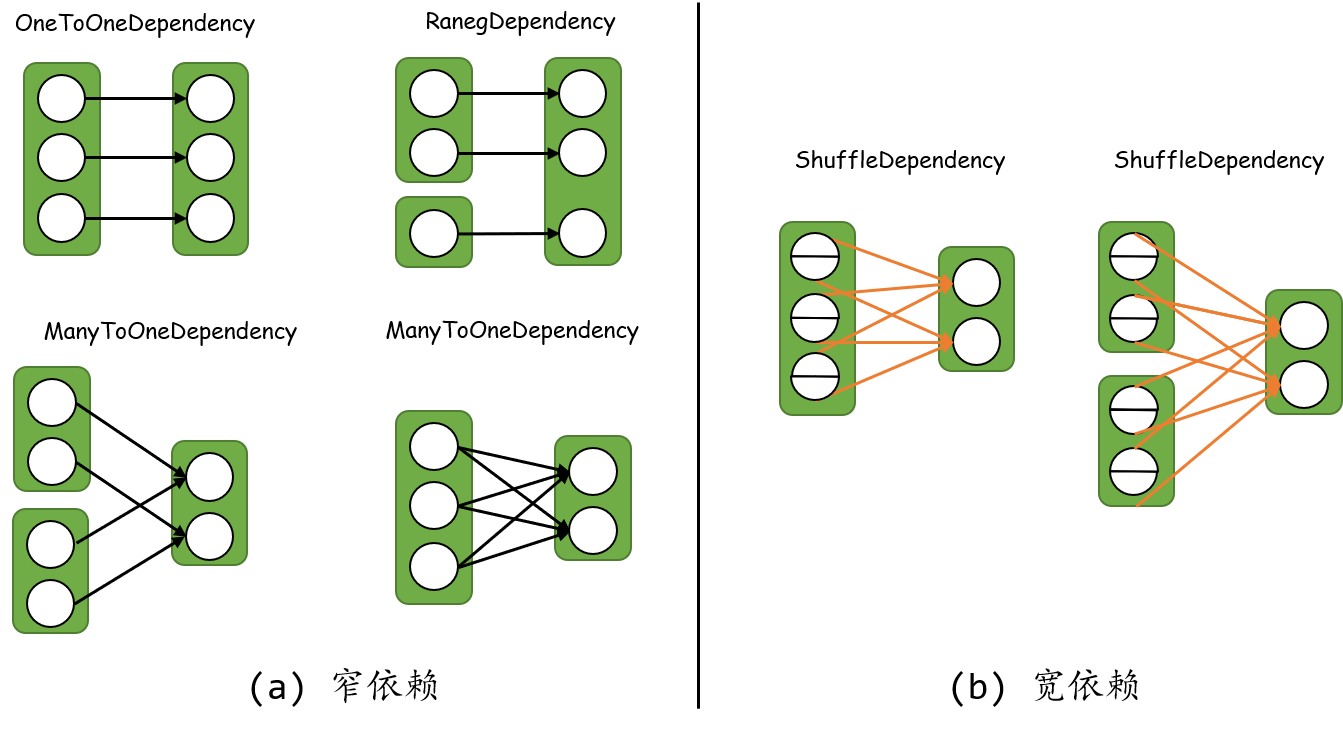
\includegraphics[width=.95\textwidth]{pics/RDD-Dependency.png}
	\caption{RDD 中的依赖关系}
	\label{fig:rdd_den}
\end{figure}

\subsubsection{窄依赖}

子 RDD 中每个分区都依赖于父 RDD 中的一部分分区, 如 Fig.\ref{fig:rdd_den}(a) 所示. 可以分成四种窄依赖:

\begin{itemize}
	\item 一对一依赖 (OneToOneDependency). 子 RDD 和父 RDD 的分区个数相同, 且存在一一映射关系, 典型的 transformation 包括 \textit{map(), filter()};
	
	\item 区域依赖 (RangeDependency). 子 RDD 和父 RDD 的分区经过区域化后存在一一映射关系, 如 \textit{union()};
	
	\item 多对一依赖 (ManyToOneDependency). 子 RDD 中的一个分区依赖\textbf{多个父 RDD} 中的分区, 如 \textit{join()};
	
	\item 多对多依赖 (ManyToManyDependency). 子 RDD 中的一个分区依赖父 RDD 中的多个分区, 同时发父 RDD 中的一个分区被子 RDD 中的多个分区依赖, 如 \textit{cartesian()}.
\end{itemize}

ManyToOneDependency 和 ManyToManyDependency 是我参考《大数据处理框架 Apache Spark 设计与实现》引入的, 实际在 Spark 代码中并没有对这两种依赖进行命名.

\subsubsection{宽依赖}

子 RDD 中的分区依赖父 RDD 中每个分区的一部分, 如 Fig.\ref{fig:rdd_den}(b) 所示. 典型的宽依赖 transformation 包括 \textit{groupByKey(), partitionBy(), reduceByKey()} 等.

窄, 宽依赖的区别在于子 RDD 的各个分区是否\textbf{完全依赖} (\textcolor{red}{指父 RDD 中的一个分区不需要进行划分就可以流入子 RDD 的分区中})父 RDD 的一个或多个分区. 

\textcolor{red}{为什么要进行数据以来关系进行分类呢?} 1) 明确 RDD 分区之间的数据依赖关系, 执行时可以确定从哪里获得数据, 输出数据到哪; 2) 有利于生成物理执行计划. 同一 stage 内的窄依赖的分区可以并行执行, 宽依赖需要进行 Shuffle. 

\subsubsection{数据分区方法}

RDD 内部的数据是如何分区的. Spark 中的分区方法:

\begin{itemize}
	\item 水平划分. 按照 record 的索引进行划分;
	
	\item Hash 划分 (HashPartitioner). 使用 record 的 Hash 值对数据进行划分;
	
	\item Range 划分 (RangePartitioner). 按照元素的序关系进行划分;
	
	\item 自定义划分. 按照自己的需求实现 Partitioner.
\end{itemize}



\subsection{物理执行计划}

有了逻辑执行计划 (即 RDD 组成的数据依赖有向无环图), 该怎么去执行呢? 物理执行计划即 Spark 是如何完成计算的. Spark 以逻辑执行计划为基础生成物理执行计划. 

\subsection{Shuffle 机制}